\documentclass[10pt]{article}

\usepackage{amsfonts,amssymb}
\usepackage{amsmath}
\usepackage[utf8]{inputenc}
\usepackage[english,russian]{babel}
\usepackage{graphicx}
\usepackage{mathtools}

\newcommand{\argmin}{\mathop{\rm arg\,min}\limits}
\newcommand{\argmax}{\mathop{\rm arg\,max}\limits}
\newcommand{\sign}{\mathop{\rm sign}\limits}
\newcommand{\cond}{\mspace{3mu}{|}\mspace{3mu}}
\def\RR{\mathbb{R}}
\usepackage{enumitem}

\textheight=220mm
\textwidth=160mm

\title{Школа анализа данных\\Машинное обучение, часть 2\\Домашнее задание №1}
\author{}
\date{}

\begin{document}


\voffset=-20mm
\hoffset=-17mm
\font\Got=eufm10 scaled\magstep2 \font\Got=eufm10


\maketitle

Решите предложенные задачи. Решения необходимо оформить в виде PDF документа. Каждая задача должна быть подробно обоснована, задачи без обоснования не засчитываются. Решения пишутся в свободной форме, однако так, чтобы проверяющие смогли разобраться. Если проверяющие не смогут разобраться в решении какой-нибудь задачи, то она автоматически не засчитывается. Дедлайн очников 15 октября 2018 09:00MSK, дедлайн заочников и филиалов +2 суток.


\bigskip

\textbf{Задача 1 (0.5 балла) Нейронные сети.}


Дана выборка из двух концентрических окружностей:
\begin{center}
    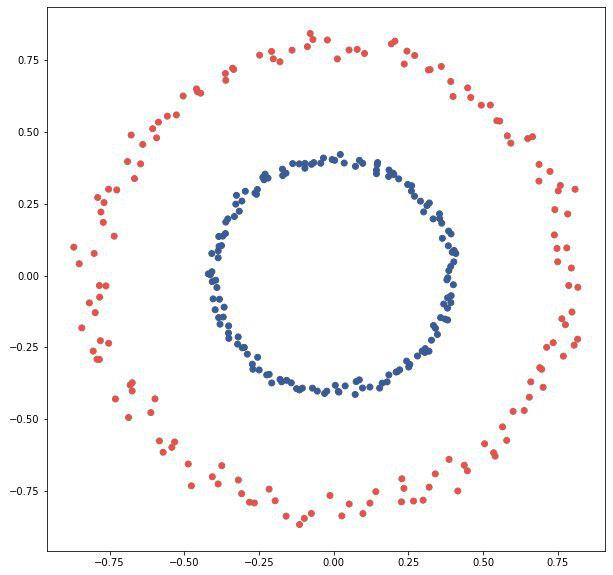
\includegraphics[width=200px]{circles.jpg}
\end{center}

Допустим, что для классификации нужно обучить нейронную сеть — причем доступны только следющие слои: линейный $L(n, m)$ ($Wx+b,~x\in\mathbb{R}^{n},~b\in\mathbb{R}^{m}$)  и активация $A$  (сигмоида или $\tanh$), которые разрешено последовательно ставить друг после друга.

Вопрос: какие из приведенных ниже архитектур будут способны разделить выборку со 100\% accuracy? Почему?

\begin{enumerate}
    \item $L(2, 2)\to A\to L(2, 1)$
    \item $L(2, 2) \to A \to L(2, 2) \to A \to L(2, 1)$
    \item $L(2, 3) \to L(3, 1)$
    \item $L(2, 3) \to A \to L(3, 1)$
    \item $L(2, 3) \to L(3, 3) \to L(3, 1)$
\end{enumerate}


\bigskip

\textbf{Задача 2 (1.5 балла) Нейронные сети, back-prop.}

    Рассмотрим двуслойную полносвязную нейронную сеть, применяемую для задачи классификации.
    На вход нейронной сети подается вектор признаков~$x$ размерности $n$, полносвязный слой с матрицей весов~$W$ размерности ${n\times d}$ преобразует вектор~$x$ в скрытое представление~$h$ некоторой размерности~$d$:
    \[
    h = x W
    \]
    Функции активации нет, еще один полносвязный слой c матрицей весов~$W'$ размерности ${d \times m}$ преобразует скрытое представление в вектор оценок~$a$ принадлежности к каждому классу.
    Чтобы получить из этих оценок вероятности, используется softmax. Например, вероятность того, что объект, описываемый вектором признаков~$x$, относится к классу $j$ согласно нейронной сети выглядит так:
    \[
    p_j = \frac{\exp(a_j)}{\sum_{k=1}^{m} \exp(a_k)}
    \]
    В качестве функции потерь используется cross-entropy loss:
    \[
    \mathcal{L} = - \sum_{j=1}^{m} y_j \log p_j, 
    \]
    где $y$ -- one-hot encoding истинной метки объекта.
    
    Итак, мы полностью описали проход по нейронной сети вперед: как по входному вектору~$x$ найти вероятности классов~$p_j$ и вычислить значение функции потерь, зная ответ~$y$ на рассматриваемом объекте. Опишите обратный проход по нейронной сети: выпишите формулы изменения матриц весов~$W$ и~$W'$ в стохастическом градиентном спуске для метода обратного распространения ошибки (backpropagation).

\bigskip
\newpage
\textbf{Задача 3.  Нейронные сети, инициализация весов.}

Рассмотрим полносвязный слой нейронной сети с матрицей весов $W$ и свободным членом $b$, получающий на вход вектор $x$ размерности $n$ и вычисляющиющий скрытое представление размерности~$m$
$$h = Wx + b.$$ 
Предложите, из какого невырожденного вероятностного распределения надо выбирать веса $W$ и $b$, чтобы активации $h$ имели нормальное распределение $N(0,\sigma^2)$, если
\begin{enumerate}[label=(\alph*)]
\item \textbf{(1 балл)} Все признаки независимы и распределены по стандартному нормальному закону.
\item \textbf{(2 балла)} Все признаки независимы и распределены равномерно от $0$ до $a$.

Распределения $W$ и $b$ не обязаны совпадать, они могут быть из разных семейств.
\end{enumerate}


\bigskip

\textbf{Задача 4 (1.5 балла) Композиции алгоритмов, бустинг, AdaBoost}.

    Обозначим через~$\tilde w^{(N)}$ нормированный вектор весов
    на~$N$-й итерации алгоритма AdaBoost.
    Покажите, что взвешенная ошибка базового классификатора~$b_N$
    относительно весов со следующего шага~$\tilde w_i^{(N + 1)}$
    равна~$1/2$:
    \[
        \sum_{i = 1}^{\ell}
            \tilde w_i^{(N + 1)}
            [b_N(x_i) \neq y_i]
        =
        \frac{1}{2}.
    \]
    
\bigskip


\textbf{Задача 5 (2 балла) Градиентный бустинг}.
    ~

    \begin{enumerate}

        
        \item Какой функции потерь будет соответствовать градиентный бустинг, который на каждой итерации настраивается на разность между вектором истинных меток и текущим вектором предсказанных меток?
        
        \item Градиентный бустинг обучается на пяти объектах с функцией потерь для одного объекта
        \[
            \mathcal{L}(\tilde y, y) = (\tilde y - y)^4.
        \]
        На некоторой итерации полученная композиция дает ответ $(5, 10, 6, 3, 0)$. На какой вектор ответов будет настраиваться следующий базовый алгоритм, если истинный вектор ответов равен $(6, 8, 6, 4, 1)$? 
        
        \item Рассмотрим задачу бинарной классификации,~$Y = \{0, 1\}$.
    Будем считать, что все алгоритмы из базового семейства~$\mathcal{A}$
    возвращают ответы из отрезка~$[0, 1]$, которые можно интерпретировать
    как вероятности принадлежности объекта к классу~$1$.
    В качестве функции потерь возьмем отрицательный
    логарифм правдоподобия~(negative log-likelihood):
    \[
        L(y, z)
        =
        -\bigl(
        y \log z
        +
        (1 - y) \log(1 - z)
        \bigr),
    \]
    где~$y$~--- правильный ответ, а~$z$~--- ответ алгоритма.

    Выпишите формулы для поиска базовых алгоритмов~$b_n$
    и коэффициентов~$\gamma_n$ в градиентном бустинге.
    \end{enumerate}
\bigskip



\bigskip
\textbf{Задача 6 (1.5 балла) Композиции, устойчивость к шуму}.
    ~

    \begin{enumerate}
      \item Рассмотрим алгоритм AdaBoost~--- бустинг с экспоненциальной функцией потерь \\
      $$\mathcal{L}(M)=\exp(-M),$$
где $M$ — отступ объекта. Покажите, что алгоритм неустойчив к шуму, т.е. возможен неограниченный рост отношения весов шумовых объектов по отношению к весам пороговых объектов.
      \item Покажите, что бустинг с логистической функцией потерь\\
      $$\mathcal{L}(M) = \log (1+\exp(-M))$$
устойчив к шуму в описанном выше смысле смысле.
    \end{enumerate}
    
    ~
    
    Примечание. Пороговые объекты~--- это те, для которых значение отступа положительно и порядка нуля, то есть они лежат близко к границе между классами и в своем классе. Шумовые объекты лежат глубоко в чужом классе, на них отступ принимает большие отрицательные значения. 
\bigskip




\end{document}
